%%%%%%%%%%%%%%%%%%%%%%%%%%%%%%%%%%%%%%%%%%%%%%%%%%%%%%%%%%%%%%%%%%%%%%%%%%%%%
%
% Bayesian prediction of luminosity distribution based on one simulation run:
% An example from TARDIS
%
%%%%%%%%%%%%%%%%%%%%%%%%%%%%%%%%%%%%%%%%%%%%%%%%%%%%%%%%%%%%%%%%%%%%%%%%%%%%%
\documentclass[11pt]{article}
\usepackage[utf8]{inputenc}

\usepackage[a4paper, left=20mm, right=20mm, top=25mm, bottom=25mm]{geometry}
\usepackage[numbers]{natbib}
\usepackage{hyperref}
\synctex=1

\usepackage[colorinlistoftodos]{todonotes} % Use 'disable' to remove todos in final version
\newcommand{\fred}[1]{\todo[color=orange!40,inline]{#1}} %
\newcommand{\checked}{\todo[color=green,noline]{\checkmark}} %
\newcommand{\checkedl}{\todo[color=brown]{\checkmark}} %
\newcommand{\hans}[1]{\todo[color=yellow!30,inline]{#1}} %
\newcommand{\hanslong}[2][]{\todo[%bordercolor=red,
  color=white,inline,caption={2do}, #1]{
    \begin{minipage}{\textwidth} #2\end{minipage}}} %

%% CHANGE THIS DATE AS YOU MODIFY THE FILE
\newcommand{\vdate}{160510}
\pagestyle{myheadings}
\markboth{Version \vdate} {Version \vdate}
\parindent=0mm
\def\pp{\hfill\par \vspace{\baselineskip}}
%% \def\pp{}
%%%%%%%%%%%%%%%%%%%%%%%%%%%%%%%%%%%%%%%%%%%%%%%%%%%%%%%%%%%%%%%%%%%%%%%%%%%%%
\usepackage{bm,amssymb,amsfonts,amsmath}  % bold math symbols, AMStex
\usepackage{graphicx}    % standard graphics
%%%%%%%%%%%%%%%%%%%%%%%%%%%%%%%%%%%%%%%%%%%%%%%%%%%%%%%%%%%%%%%%%%%%%%%%%%%%%
\newcommand{\lleq}[1]{\label{#1} }
% TO REMOVE THE LABEL LETTERS FROM THE EQUATION DISPLAY, COMMENT OUT THIS LINE:
\renewcommand{\lleq}[1]{\label{#1} {\scriptstyle {\rm (#1)}} \hspace*{2ex} }
% \renewcommand{\labelenumi}{\arabic{section}.\arabic{subsection}.\arabic{enumi}}
% \renewcommand{\thesubsubsection}{\arabic{subsubsection}}

\newcounter{mnumi}
\newenvironment{mnumerate}{
  \begin{list}{\arabic{mnumi}.}
    {\usecounter{mnumi} \setlength{\itemsep}{0pt}
      \setlength{\leftmargin}{3ex}
    }
  }
  {\end{list}}

\newenvironment{mtemize}{
  \begin{list}{$\bullet$}
    {\setlength{\itemsep}{0pt}
     \setlength{\leftmargin}{3ex}
    }
  }
  {\end{list}}

\newcommand{\hmod}  {{\mathcal{H}}}  % Model
\newcommand{\ldef}{\;{:}{=}\;}
\newcommand{\rdef}{\;{=}{:}\;}
\newcommand{\realnumbers}{\mathbb{R}}
\newcommand{\integers}{\mathbb{Z}}
\newcommand{\cond}{\,|\,}
\newcommand{\NBD}{\mathrm{NB}}
\newcommand{\var}{\mathrm{var}}

\newcommand{\smA}{{\scriptscriptstyle A}}
\newcommand{\smB}{{\scriptscriptstyle B}}
\newcommand{\smH}{{\scriptscriptstyle H}}
\newcommand{\smK}{{\scriptscriptstyle K}}
\newcommand{\smL}{{\scriptscriptstyle L}}
\newcommand{\smM}{{\scriptscriptstyle M}}
\newcommand{\smN}{{\scriptscriptstyle N}}
\newcommand{\smR}{{\scriptscriptstyle R}}

\newcommand{\smo}{{\scriptscriptstyle 1}}
\newcommand{\smt}{{\scriptscriptstyle 2}}
\newcommand{\smr}{{\scriptscriptstyle 3}}
\newcommand{\smf}{{\scriptscriptstyle 4}}
\newcommand{\smv}{{\scriptscriptstyle 5}}
\newcommand{\smx}{{\scriptscriptstyle 6}}
\newcommand{\sms}{{\scriptscriptstyle 7}}
\newcommand{\sme}{{\scriptscriptstyle 8}}
\newcommand{\smn}{{\scriptscriptstyle 9}}

\newcommand{\bma}{{\bm{a}}}
\newcommand{\bmb}{{\bm{b}}}
\newcommand{\bmc}{{\bm{c}}}
\newcommand{\bmd}{{\bm{d}}}
\newcommand{\bme}{{\bm{e}}}
\newcommand{\bmf}{{\bm{f}}}
\newcommand{\bmg}{{\bm{g}}}
\newcommand{\bmh}{{\bm{h}}}
\newcommand{\bmi}{{\bm{i}}}
\newcommand{\bmj}{{\bm{j}}}
\newcommand{\bmk}{{\bm{k}}}
\newcommand{\bml}{{\bm{\ell}}}
\newcommand{\bmm}{{\bm{m}}}
\newcommand{\bmn}{{\bm{n}}}
\newcommand{\bmo}{{\bm{o}}}
\newcommand{\bmp}{{\bm{p}}}
\newcommand{\bmq}{{\bm{q}}}
\newcommand{\bmr}{{\bm{r}}}
\newcommand{\bms}{{\bm{s}}}
\newcommand{\bmt}{{\bm{t}}}
\newcommand{\bmu}{{\bm{u}}}
\newcommand{\bmv}{{\bm{v}}}
\newcommand{\bmw}{{\bm{w}}}
\newcommand{\bmx}{{{\bm{x}}}}
\newcommand{\bmy}{{\bm{y}}}
\newcommand{\bmz}{{\bm{z}}}
\newcommand{\bmA}{{\bm{A}}}
\newcommand{\bmB}{{\bm{B}}}
\newcommand{\bmC}{{\bm{C}}}
\newcommand{\bmD}{{\bm{D}}}
\newcommand{\bmE}{{\bm{E}}}
\newcommand{\bmF}{{\bm{F}}}
\newcommand{\bmG}{{\bm{G}}}
\newcommand{\bmH}{{\bm{H}}}
\newcommand{\bmI}{{\bm{I}}}
\newcommand{\bmJ}{{\bm{J}}}
\newcommand{\bmK}{{\bm{K}}}
\newcommand{\bmL}{{\bm{L}}}
\newcommand{\bmM}{{\bm{M}}}
\newcommand{\bmN}{{\bm{N}}}
\newcommand{\bmO}{{\bm{O}}}
\newcommand{\bmP}{{\bm{P}}}
\newcommand{\bmQ}{{\bm{Q}}}
\newcommand{\bmR}{{\bm{R}}}
\newcommand{\bmS}{{\bm{S}}}
\newcommand{\bmT}{{\bm{T}}}
\newcommand{\bmU}{{\bm{U}}}
\newcommand{\bmV}{{\bm{V}}}
\newcommand{\bmW}{{\bm{W}}}
\newcommand{\bmX}{{\bm{X}}}
\newcommand{\bmY}{{\bm{Y}}}
\newcommand{\bmZ}{{\bm{Z}}}

\newcommand{\bmalpha}{{\bm{\alpha}}}
\newcommand{\bmbeta}{{\bm{\beta}}}
\newcommand{\bmchi}{{\bm{\chi}}}
\newcommand{\bmdelta}{{\bm{\delta}}}
\newcommand{\bmepsilon}{{\bm{\varepsilon}}}
\newcommand{\bmphi}{{\bm{\phi}}}
\newcommand{\bmgamma}{{\bm{\gamma}}}
\newcommand{\bmeta}{{\bm{\eta}}}
\newcommand{\bmiota}{{\bm{\iota}}}
\newcommand{\bmkappa}{{\bm{\kappa}}}
\newcommand{\bmlambda}{{\bm{\lambda}}}
\newcommand{\bmmu}{{\bm{\mu}}}
\newcommand{\bmnu}{{\bm{\nu}}}
\newcommand{\bmomega}{{\bm{\omega}}}
\newcommand{\bmpi}{{\bm{\pi}}}
\newcommand{\bmpsi}{{\bm{\psi}}}
\newcommand{\bmrho}{{\bm{\rho}}}
\newcommand{\bmsigma}{{\bm{\sigma}}}
\newcommand{\bmtau}{{\bm{\tau}}}
\newcommand{\bmtheta}{{\bm{\theta}}}
\newcommand{\bmupsilon}{{\bm{\upsilon}}}
\newcommand{\bmxi}{{\bm{\xi}}}
\newcommand{\bmzeta}{{\bm{\zeta}}}

\newcommand{\refeq}[1]{Eq.~(\ref{#1})}
\newcommand{\reffig}[1]{Fig.~\ref{fig:#1}}
\newcommand{\refsec}[1]{Sec.~\ref{sec:#1}}

\DeclareMathOperator{\GammaDist}{Gamma}
\newcommand{\Kalpha}{{K_\alpha}}
\newcommand{\Kbeta}{{K_\beta}}
\newcommand{\npack}{n_p}
\newcommand{\lmax}{\ell_{\rm max}}
\newcommand{\Lmax}{L_{\rm max}}
\newcommand{\rmdx}[1]{\mbox{d} #1 \,} % differential
\newcommand{\firstDeriv}[1]{\frac{\partial}{\partial #1}}
\newcommand{\secDeriv}[1]{\frac{\partial^2}{\partial #1^2}} % second partial derivative
\newcommand{\secPartial}[2]{\frac{\partial^2}{\partial #1 \, \partial #2}} % second partial derivative
\newcommand{\tardis}{TARDIS}

%%%%%%%%%%%%%%%%%%%%%%%%%%%%%%%%%%%%%%%%%%%%%%%%%%%%%%%%%%%%%%%%%%%%%%%%%%%%%
\begin{document}

\begin{center}
  \textbf{\Large Bayesian prediction of supernova luminosity  distributions}\\[8pt]
  \textbf{\Large based on simulation output: An example from \tardis}\\[12pt]
\end{center}

\textbf{Abstract} TODO\\

\section{Introduction} \label{sec:intro}

\begin{itemize}
  \item radiative transfer
  \item get uncertainty from single run
  \item cover case when few packets in a bin
\end{itemize}

\section{Notation} \label{sec:notation}

We consider a computer simulation that, given input parameters
$\bmtheta$ and a random-number seed, produces a set of simulated data
$ S = \{ (\nu_j, \ell_j): j=1\dots\npack \}$ consisting of $\npack$
packets, each with a frequency and a luminosity. We distinguish
between a random variable $L$ and its concrete realization $\ell$.  To
learn about $\bmtheta$, we need to compare to data from a telescope
available as luminosities in frequency bins, $D = \{ ( \nu_b, \ell_b):
b=1 \dots B\}$. The natural estimate from a single simulation is to
add up the luminosities of all packets in a bin.  With a different
seed but identical $\bmtheta$, both the number of packets in the bin
and their luminosities could be different. Our goal is to estimate the
distribution based on a \emph{single} simulation without recourse to
expensive repetitions or asymptotic approximations; i.e., we seek
$P(L_b \cond \nu_b, \npack, \bmnu, \bml )$. In an actual physics
analysis, one would proceed to plug in the observed value $\ell_b$ and
perform an analysis to learn about $\bmtheta$. But here we focus on
the specific problem of $P(L_b \cond \nu_b, \npack, \bmnu, \bml )$ and
hence omit $\bmtheta$ throughout.

Various features, for example absorption lines, usually make it
difficult to explicitly model the spectrum---the luminosity as a
function of frequency. In a binned analysis, we can avoid these
difficulties associated to modeling $n_b$. Our approach, however,
requires an explicit expression of how the distribution of the
luminosity of a single packet in our simulation changes with $\nu$. It
is this crucial piece of information that allows us to extend previous
methods \fred{Refs: Zech, maybe others, too} in dealing with the
extreme cases when the number of packets in a bin, $n_b$, is one or
even zero.

\section{Model} \label{sec:model}

We consider the total number of packets $\npack$ fixed, for example
chosen by a user. In contrast, the number of packets in a bin, $n_b$
is a realization of a random variable $N_b$ which we assume to follow
a Poisson distribution. With this assumption, we neglect bin-by-bin
correlations and treat each bin independently which allows us to focus
on a single bin and to drop the subscript $b$ in the remainder. Hence
\begin{align}
  \lleq{caa}
  p(N\cond\lambda) &= \frac{e^{-\lambda}\lambda^N}{N!}
  \qquad N = 0,1,\ldots,\infty ,
\end{align}
where the dependency of the Poisson mean $\lambda>0$ on $\nu$ is of no
concern to us. Let $\bmL$ denote the collection of luminosities of
packets in a certain bin. The total luminosity in that bin is then
given by
\begin{align}
  \lleq{cab}
  L = \sum_{j=1}^{N} L_j\,.
\end{align}
We assume that each $L_j$ has a distribution depending on $\nu$ and
other parameters $\bmphi$ and that each packet is statistically
independent. Since $N$ is random, $L$ is said to follow a compound
Poisson process. The joint distribution then is
\begin{align}
  \lleq{cac}
  (N,\bmL) &\ \sim\ p(N,\bmL\cond \bmphi,\lambda, \nu)
  = p(\bmL\cond N,\bmphi, \nu)\; P(N\cond \lambda) = \prod_{j=1}^N p(L_j\cond \bmphi, \nu) \; P(N\cond \lambda),
\end{align}
where we used that the Poisson term does not depend on $\nu$
explicitly. In general, the distribution of $L_j$ could be a of a
different functional form in each bin. For simplicity, we assume it is
identical but may depend on parameters that differ from bin to bin. In
practice, the distribution of packets does not change abruptly with
frequency. We therefore assume that any parameter needed to fully
specify $p(L_j)$ is given explicitly as a continuous function of $\nu$
and the unknown parameters $\bmphi$. This allows us to use a small
number of parameters to describe $P(L)$ across the entire frequency
range and in turn lets us determine $\bmphi$ from fitting all
simulated packets simultaneously whereas $\lambda$ is given only by
the packets in a bin.

Our goal of predicting $L$ in bin $b$ given the simulation output
$(\npack,\bml, \bmnu)$ is captured in the probability $p(L\cond \nu,
\npack,\bml, \bmnu)$ with all relevant parameters integrated out using
the law of total probability.  To simplify the treatment, we assume
that the frequency bins are narrow or equivalently that $p(L \cond
\nu, \npack, \bml, \bmnu)$ does not vary within a bin. This implies
that all every sample $L_j$ in the bin follows the same distribution.
As the reference frequency, we choose the bin center.

We first note from \refeq{caa} that $N$ does not depend on $\bml$ at
all and only indirectly depends on $\bmnu$ through $n$. Since $L$ is
fully determined by $(N,\bmL)$, it does not depend on
$(\npack,\bml,\bmnu)$, i.e.
\begin{align}
  \lleq{pmi}
  p(L\cond N,\bmL,\nu,\npack,\bml, \bmnu)
  = p(L\cond N, \bmL)
  &= \delta(L - \textstyle\sum_{j=1}^N L_j),
\end{align}
\fred{Uniform order: $\nu$ first, then $\ell$, compare to $S$}
where the $L_j$ are assumed to occur at $\nu$.  Using the law of total
probability repeatedly, we can write the desired distribution
\fred{Discuss $N=0$ case somewhere}
\begin{align}
  \lleq{pmj}
  p(L\cond \nu, \npack,\bml, \bmnu)
  &= \sum_N p(N\cond \nu, \npack,\bml, \bmnu) \, p(L\cond N,\nu, \npack,\bml, \bmnu) \\
  \lleq{pmjb}
  &= \sum_N p(N\cond n)\,\int \rmdx{\bmL} p(L\cond N,\bmL,\nu, \npack,\bml, \bmnu)\, p(\bmL\cond N,\nu, \npack,\bml, \bmnu)
  \\
  \lleq{pmjc}
  &= \sum_N p(N\cond n)\,\int \rmdx{\bmL} \delta(L - \textstyle\sum_{j=1}^N L_j)
  \, p(\bmL\cond N,\nu, \npack,\bml, \bmnu)
\end{align}
The dependence on the simulation output $(\npack,\bml, \bmnu)$ enters
through $p(\bmL\cond N,\npack,\bml, \bmnu)$ in terms of the parameters
$\bmphi$ of $p(\bmL\cond N,\bmphi)$,
\begin{align}
  p(\bmL\cond N,\nu, \npack,\bml, \bmnu)
  &= \int \rmdx{\bmphi} p(\bmL\cond \bmphi,N, \nu, \npack,\bml, \bmnu)\,p(\bmphi\cond N,\nu, \npack,\bml, \bmnu) \\
  \lleq{pmk}
  &= \int \rmdx{\bmphi} p(\bmL\cond \bmphi, N, \nu)\,p(\bmphi\cond N,\nu, \npack,\bml, \bmnu).
\end{align}
because $\bmL$ is fully determined by $N,\bmphi, \nu$ and hence
independent of $\npack,\bml, \bmnu$.  With Bayes' theorem we learn about
$\bmphi$ from the simulation output
\begin{align}
  \lleq{pmkb}
  p(\bmphi\cond N,\nu, \npack,\bml, \bmnu) &=
  \frac{p(\bml\cond \bmphi, N,\nu, \npack,\bmnu)\,p(\bmphi\cond N,\nu, \npack,\bmnu)} %
  {\int \rmdx{\bmphi} p(\bml\cond \bmphi,N,\nu, \npack,\bmnu)\,p(\bmphi\cond N,\nu, \npack,\bmnu)}.
\end{align}
By using a multiplicity- and frequency-independent prior for $\bmphi$,
\begin{align}
  \lleq{pml}
  p(\bmphi\cond N,\nu, \npack,\bmnu) &= p(\bmphi),
\end{align}
and by recognizing that $\bml$ is independent of $N$ and $\nu$
\begin{align}
  \lleq{pmla}
  p(\bml\cond \bmphi,N,\nu, \npack,\bmnu) = p(\bml\cond \bmphi,\npack,\bmnu)
\end{align}
we can write \refeq{pmk} as
\begin{align}
  \lleq{pmn}
  p(\bmL\cond N,\nu, \npack,\bml, \bmnu)
  &= \int \rmdx{\bmphi} p(\bmL\cond N,\bmphi)\, %
  \frac{p(\bml\cond \bmphi, \npack, \bmnu)\,p(\bmphi)} %
  {\int \rmdx{\bmphi} p(\bml\cond \bmphi,\npack,\bmnu)\,p(\bmphi)} \\
  \lleq{pmo}
  &= \frac{1}  {p(\bml\cond \npack, \bmnu)} %
  \int \rmdx{\bmphi} p(\bmL\cond \bmphi, N)\, %
  p(\bml\cond \bmphi, \npack,\bmnu)\,p(\bmphi)
\end{align}
with $p(\bml\cond \npack, \bmnu) = \int \rmdx{\bmphi} p(\bml\cond
\bmphi, \npack,\bmnu)\,p(\bmphi)$ is the evidence in the denominator.
Inserting this into (\ref{pmjc}), we obtain the desired master equation:
\begin{equation}
  \lleq{pmp}
  \boxed{
  p(L\cond \nu, \npack,\bml, \bmnu)
  = \frac{1}{p(\bml\cond \npack, \bmnu)}
  \sum_N p(N\cond n)\,\int \rmdx{\bmL} \delta(L - \textstyle\sum_j L_j)
  \displaystyle\int \rmdx{\bmphi} p(\bmL\cond \bmphi, N, \nu) \, p(\bml\cond \bmphi,\npack,\bmnu)
  \, p(\bmphi)
  }
\end{equation}
with
\begin{align}
  \lleq{pmq}
  p(\bmL\cond \bmphi, N, \nu) &= \prod_{j=1}^N p(L_j\cond \bmphi, \nu), \\
  \lleq{pmr}
  p(\bml\cond \bmphi,\npack,\bmnu) &= \prod_{j=1}^{\npack} p(\ell_j\cond \bmphi, \nu_j)
\end{align}
and $p(\cdot \cond \bmphi, \cdot)$ is the same function in both
equations.  In the next section, we compute the general result for
$P(N \cond n)$. Equation \refeq{pmp} then implies that once we specify
the prior $p(\bmphi)$ and the likelihood $p(L_j\cond \bmphi, \nu)$, we
have a prediction for $L$ which takes into account all possible $N$,
$\lambda$ and $\bmphi$. Both choices depend on the simulation at hand
but a general consideration to render our approach tractable is that
the distribution of a single packet luminosity $P(L_j \cond \bmphi,
\nu)$ should be such that the integral over $\bmL$ has a closed-form
solution. In other words, for a given distribution of $L_j$, the
distribution of $L = \sum_N L_j$ should be known.
%  An important special case is the class of \emph{stable}
% distributions.

\subsection{Predicting the number of packets in a bin}
\fred{Show reference Poisson analysis here of before?}

We use Bayes' theorem to find the posterior distribution for $\lambda$
given data $n$ and the Poisson hypothesis
\begin{align}
  \lleq{pmd}
  p(\lambda\cond n) %
  &= \frac{p(n\cond\lambda)\,p(\lambda)} {p(n)}
  \ =\ \frac{p(n\cond\lambda)\,p(\lambda)} %
  {\int \rmdx{\lambda} p(n\cond\lambda)\,p(\lambda)}
\end{align}
to find the posterior predictive of $N$ given $n$ taking into account
all possible values of $\lambda$,
\begin{align}
  \lleq{pme}
  p(N\cond n)
  &= \int \rmdx{\lambda}p(N,\lambda\cond n)
  \ =\ \int \rmdx{\lambda} p(N\cond\lambda, n)\,p(\lambda\cond n)
  \ =\ \frac{\int \rmdx{\lambda} p(N\cond\lambda)\,p(n\cond\lambda)\,p(\lambda)}
  {\int \rmdx{\lambda} p(n\cond\lambda)\,p(\lambda)}
\end{align}
where $p(N\cond\lambda,n) = p(N\cond\lambda)$ is independent of $n$.
A common choice is the prior
\begin{align}
  \lleq{pmf}
  p(\lambda) = c\lambda^{-a},
\end{align}
where $a=0$ gives the uniform prior\footnote{For a uniform prior, the
  case $a{=}0$, we require of course a maximum $\lambda_{\rm max}$. As
  long as $\lambda_{\rm max}$ is large enough, the integral can
  effectively be taken to infinity.} and $a=1/2$ gives the Jeffreys
and reference prior. Both choices lead to an improper prior but the
posterior predictive is proper provided that $n>0$ or $N>0$.  The
standard results for the evidence and the posterior predictive are
\begin{align}
  \lleq{pmg}
  p(n) &= %
  \int_0^\infty d\lambda\, p(n\cond\lambda)\,p(\lambda)
  \ =\
  c \int_0^\infty d\lambda\, \frac{e^{-\lambda}\,\lambda^{n-a}}{n!}
  \ =\ c\frac{(n-a)!}{n!} \, ,
  \\
  \lleq{pmh}
  p(N\cond n) %
  &= \frac{n!}{(n-a)!} \int_0^\infty d\lambda\,
  \frac{e^{-2\lambda} \lambda^{N+n-a}}{N!\, n!}
  \ =\ \frac{(N+n-a)!}{N!\,(n-a)!\,2^{N+n+1-a}} \, .
\end{align}

\section{Example application: \tardis} \label{sec:example}

 The \tardis{} packages simulates supernovae with \fred{Wolfgang's
  favorite description of his package}. Here we focus on the real
packets as opposed to the virtual packets output by tardis.

% Based on staring at the distribution of luminosities,
To apply \refeq{pmp}, we first need to choose $P(L_j \cond \bmphi,
\nu)$. A histogram of the luminosities from a \tardis{} run indicates
a strongly skewed distribution with a single mode that is close to but
not at the sharp end point $\lmax$. There is a long tail for small
$\ell$. These features can be accomodated by a $\GammaDist$
distribution with shape parameter $\alpha$ and rate
parameter $\beta$
\begin{align}
  \lleq{gma}
  \GammaDist(x | \alpha, \beta) = \frac{\beta^\alpha}{\Gamma(\alpha)} x^{\alpha-1} e^{-\beta x}\, , \; x > 0 .
\end{align}
Since $\ell$ seems bounded from above, we have to transform the data.
We first take the largest luminosity of all \tardis{} packets across the
entire frequency range and increase it slightly to avoid numerical
difficulties at the end point
\begin{align}
  \lleq{gme}
  \lmax \equiv (1+\epsilon) \times \max_j \ell_j,
\end{align}
where $ \epsilon=10^{-6}$.  We assume the total number of samples
across all bins is large, hence the effect of considering $\lmax$ a
constant independent of the data is negligible. We checked that
leaving $\lmax$ as a free parameter in a fit gave equivalent
results. We define
\begin{align}
  \lleq{gmf}
  x_j \equiv 1- \frac{\ell_j}{\lmax} > 0
\end{align}
and similarly for $L \to X$, then we infer $P(X \cond \nu, \npack,
\bmx, \bmnu)$. If necessary, we transform back to a probability
density in $L$ via
\begin{align}
  \lleq{gmg}
  p(L  \cond \nu,  \npack, \bml, \bmnu) = p(X  \cond \nu,  \npack, \bmx, \bmnu) \frac{1}{\lmax} \,.
\end{align}
To simplify the numerics, we also rescale the frequencies by a fixed
constant from $\mathcal{O}(10^{15})$ to $\mathcal{O}(1)$.  A major
numerical simplification arises because of the $L \to X$
transformation. Rewriting the master equation~(\ref{pmp}) formally as
\begin{align}
  \lleq{gmh}
  p(L  \cond \nu,  \npack, \bml, \bmnu) = \sum_{N} p(N \cond \nu,  n) p(L \cond N,
\nu, \npack, \bml, \bmnu)
\end{align}
we see that the right-hand side is a mixture density. In our
application, the distribution of a single packet luminosity is narrow
in the sense that the standard deviation relative to the mean is at
the percent level. This implies that $p(L \cond \nu, \npack, \bml,
\bmnu)$ has one mode from each $N$ and all modes are clearly
separated. The transformation $L \to x$ effects a strong overlap
between the distributions $p(X \cond N, \nu, \npack, \bmx, \bmnu)$
with similar $N$, so $p(X \cond \nu, \npack, \bmx, \bmnu)$ can be well
approximated by a unimodal distribution; see \reffig{hedgehog}.

\begin{figure}[ht]
  \centering
  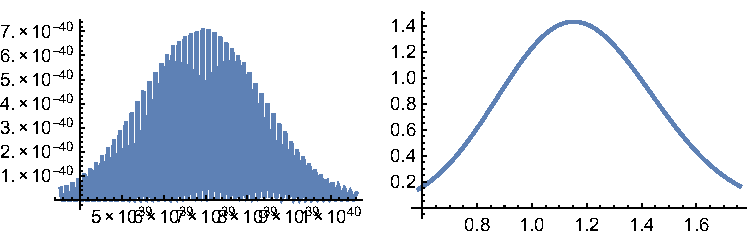
\includegraphics[width=0.48\textwidth]{hedgehog}
  \caption{Left: Prediction $p(L \cond  \nu,  \npack, \bml, \bmnu)$, right: $p(x \cond  \nu,  \npack, \bmx, \bmnu)$. I sum over $N$ in both cases. }
  \fred{I still need to pretty this up. I used the old binned approach
    with 50 samples in a bin from which I computed the mean and
    variance to plug into \refeq{gmr} but I computed the sum over $N$
    instead of the integral.}
\label{fig:hedgehog}
\end{figure}

We prefer the Gamma distribution because it is \emph{stable}; i.e.,
the sum of $N$ Gamma variates is again a Gamma variate
\begin{align}
  \lleq{gmb}
    X_j \sim \GammaDist(\alpha, \beta) \Rightarrow X \equiv \sum_{j=1}^N X_j \sim \GammaDist(N \alpha, \beta).
\end{align}
Assuming $\alpha = \alpha(\nu \cond \bmphi)$ and $\beta = \beta(\nu
\cond \bmphi)$ are functions of $\nu$ that depend on parameters
$\bmphi$, we set
\begin{align}
  \lleq{gmi}
  p(\bmX \cond \bmphi, N, \nu) &= \prod_{j=1}^N \GammaDist(X_j \cond \alpha, \beta ).
\end{align}
and equivalently $P(\bmx \cond \bmphi, \npack, \bmnu)$.  Combining
\refeq{gmb} and \refeq{gmi}, we can solve the integral
\begin{align}
  \lleq{gmc}
  \int \rmdx{\bmX} \delta(X - \textstyle\sum_j X_j)
  \,p(\bmX\cond N,\bmphi, \nu) = \GammaDist(X \cond N \alpha, \beta)
\end{align}
implying that the master equation~(\ref{pmp}) considerably simplifies
as
\begin{align}
  \lleq{gmd}
    \boxed{
    p(X\cond \nu, \npack,\bmx,\bmnu)
  = \frac{1}{p(\bmx\cond \npack, \bmnu)}
  \sum_N p(N\cond n)\, \int \rmdx{\bmphi} \GammaDist(X \cond N \alpha, \beta) % p(X \cond N, \bmphi, \nu)
  \, p(\bmx\cond \bmphi, \npack, \bmnu)
  \, p(\bmphi).
  }
\end{align}

\subsection{Linear model}

In the absence of a physical model to determine $\alpha(\nu \cond
\bmphi)$ and $\beta(\nu \cond \bmphi)$, we propose to start with a simple polynomial ansatz   $\alpha(\nu \cond \bmphi) = \sum_{k=0}^\Kalpha \alpha_k \nu^k, \beta(\nu \cond \bmphi) = \sum_{k=0}^\Kbeta \beta_k \nu^k$ such that
\begin{align}
  \lleq{gmp}
  \bmphi = (\alpha_0, \dots \alpha_\Kalpha , \beta_0, \dots \beta_\Kbeta)
\end{align}
The usual trade off between parsimony and the ability to accurately
model the frequency dependence determines the orders of the
polynomials, $\Kalpha$ and $\Kbeta$. This is outside the scope of this
paper. Here we choose $\Kalpha = 3$ and $\Kbeta = 1$.

\subsection{Prior} \label{sec:priors}

The only missing piece to explicitly evaluate \refeq{gmd} is the prior
$p(\bmphi)$. To gain some insight, consider the standard $\GammaDist$
model with $\Kalpha = \Kbeta = 0$.
% There is a conjugate prior but
% unfortunately the normalization constant cannot be evaluated in closed
% form, so it is thus of no use for us.
How about a noninformative prior? The authors of
\cite{moala2013bayesian} present an overview of possible choices and
conclude that the point estimate given by the mode of the posterior is
nearly insensitive to the prior choice starting from around 30
independent identically distributed samples. We posit that there are
this many samples available near any $\nu$ under consideration, so the
form of the prior is not crucial for our application. But there is
some explicit prior information that we want to build into our
analysis. The distribution $p(x \cond \alpha, \beta)$ should always
vanish at the origin. This is equivalent to requiring a maximum away
from the boundary leading to $\alpha > 1$. We choose a uniform prior
on $\bmphi$ on a finite box $V$ through indicator functions
\begin{align}
  p(\bmphi) = \mathbf{1}_{\alpha(\bmphi) > 1}(\bmphi) \mathbf{1}_V(\bmphi).
\end{align}

\subsection{Numerical implementation} \label{sec:numerical}

The box $V$ is chosen by trial and error to be large enough to contain
the relevant region of $p(\bmx\cond \bmphi, \npack, \bmnu)$. For
simple functions $\alpha(\nu \cond \bmphi)$, one can find the minimum
value of $\alpha$ over the entire range of $\nu$ analytically. If this
is too complicated, we propose to require $\alpha(\nu_j \cond \bmphi)
> 1$ only at each packet frequency $\nu_j$. In the evaluation of
$p(\bmx \cond \bmphi, \npack, \bmnu)$, one has to loop over all
packets and compute $\alpha$ and $\beta$ anyways, so the constraint
imposes essentially no computational overhead.  To explicitly evaluate
\refeq{gmd}, we have to overcome the remaining two difficulties: the
integral over $\bmphi$ and the sum over $N$.

As for the former, the posterior $p(\bmphi \cond \npack, \bmx, \bmnu)$
is approximately Gaussian in $\phi$ for $\npack$ large, so we can
apply Laplace's method to perform the $\bmphi$ integrals for both the
evidence $p(\bmx \cond \npack, \bmnu)$ and the posterior mean $p(X
\cond N, \npack, \bmx, \bmnu)$. This requires the Hessian at the mode
and the gradient helps in locating the mode; the analytic expressions
are summarized in \refsec{appendix}.

Regarding the sum over $N$, we start at $N = \lfloor n-a+1 \rfloor =
\arg \max_N p(N|n)$ \fred{Actually we should say $p(N \cond n, a)$}
and continue to larger and smaller values of $N$ until the
contribution to $P(X \cond \nu, \npack, \bmx, \bmnu)$ becomes
negligible. In case the relevant contribution is from large $N$ and
$n$, we interpret $N$ as a continuous variable, replace factorials by
$\Gamma$ function in \refeq{pmh}, and apply Laplace's method to
integrate over $N$ and $\bmphi$.

\fred{Our implementation is available online on \href{https://github.com/tardis-sn/XXX}{github}}

\subsection{Graphical output}

\section{Conclusion} \label{sec:conclusion}

\section{Appendix} \label{sec:appendix}

We use the shorthand $\alpha_n \equiv \alpha(\nu_n \cond
\bmphi), \beta_n \equiv \beta(\nu_n \cond \bmphi), \alpha \equiv
\alpha(\nu \cond \bmphi), \beta \equiv \beta(\nu \cond \bmphi)$.

\subsection{Gradients} \label{sec:gradients}

\begin{align}
  \label{eq:grad-posterior}
  \left( \firstDeriv{\alpha_i}, \firstDeriv{\beta_i} \right) \log p(\bmx \cond \alpha, \beta) &=
  \left(
    \sum_n \left[ \log \beta_n - \Psi(\alpha_n) + \log x_n \right] \nu_n^i \;,
    \sum_n \left[ \frac{\alpha_n}{\beta_n} - x_n \right]\nu_n^i
  \right)
\end{align}

\begin{align}
  \label{eq:grad-prediction}
  \left( \firstDeriv{\alpha_i}, \firstDeriv{\beta_i}, \firstDeriv{N} \right) \log p(X \cond N \alpha, \beta)  &=
  \left(
    \left[ \log \beta - \Psi(N \alpha) + \log X \right] N \nu^i,
    \left[ \frac{N\alpha}{\beta} - X \right]\nu^i,
    \left[ \log \beta -\Psi(N \alpha) + \log X \right] \alpha
  \right)
\end{align}

\begin{align}
  \label{eq:grad-nb}
  \firstDeriv{N} \log p(N \cond n) = \Psi(N+n-a+1) - \Psi(N+1) - \log 2
\end{align}

\subsection{Hessians} \label{sec:hessians}

\begin{align}
  \label{eq:hess-posterior}
    - \left(
    \begin{array}{ccc}
      \secPartial{\alpha_i}{\alpha_j} & \secPartial{\alpha_i}{\beta_j}\\
      \dots & \secPartial{\beta_i}{\beta_j}
    \end{array}
  \right) \log p(\bmx \cond \alpha, \beta)
    &= \left(
    \begin{array}{cc}
      \sum_n \Psi'(\alpha_n) \nu_n^{i+j} & -\sum_n \frac{\nu_n^{i+j}}{\beta_n}\\
      \dots & \sum_n \frac{\alpha_n}{\beta_n^2} \nu_n^{i+j}
    \end{array}
  \right)
\end{align}
with $\alpha_n \equiv \alpha(\nu_n \cond \bmphi), \beta_n \equiv \beta(\nu_n \cond \bmphi)$.

 \begin{align}
  \label{eq:hess-prediction}
  & - \left(
    \begin{array}{ccc}
      \secPartial{\alpha_i}{\alpha_j} & \secPartial{\alpha_i}{\beta_j} & \secPartial{\alpha_i}{N}\\
      \dots & \secPartial{\beta_i}{\beta_j} & \secPartial{\beta_i}{N}\\
      \dots & \dots & \secDeriv{N}
    \end{array}
  \right) \log p(X \cond N \alpha, \beta)
  \\
  &=
  \left(
    \begin{array}{ccc}
      N^2 \Psi'(N \alpha) \nu^{i+j} & -\frac{N \nu^{i+j}}{\beta} & \left[ -\log \beta +\Psi(N \alpha) + N \alpha \Psi'(N \alpha) - \log X \right] \nu^{i}\\
      \dots &  \frac{N\alpha}{\beta^2} \nu^{i+j} & -\frac{\alpha}{\beta} \nu^{i} \\
      \dots & \dots & \alpha^2 \Psi'(N \alpha)
    \end{array}
  \right)
\end{align}
with $\alpha \equiv \alpha(\nu \cond \bmphi), \beta \equiv \beta(\nu \cond \bmphi)$.
\begin{align}
  \label{eq:hess-nb}
   - \secDeriv{N} \log p(N \cond n) = \Psi'(N+1) - \Psi'(N+n-a+1)
\end{align}

\bibliographystyle{plain}
\bibliography{references}


\end{document}

% Local Variables:
% compile-command:"rubber --pdf -W refs -S draft"
% End:
